
\section{Doping determination}

Figure~\ref{Fig:ResH:TSweeps} shows measurements of the in-plane resistivity, $\rho(T)$, of the samples in zero field taken in the \ac{VTI} in the Polo magnet. The mid-transition \Tc values were extracted from the plots with the error determined from the difference between the mid point and the zero resistance point. Results are listed in table~\ref{Table:ResH:TSweepFitsParams} as well as the normalised \Tc values, $T_c/T_c(\textrm{max})$, with $T_c(\textrm{max}) = \unit{36}{\kelvin}$.

\begin{figure}[htbp]
	\begin{center}
		\includegraphics[scale=0.9]{Chapter-HallBSCO/Figures/TSweeps/TSweeps}
		\caption{The in-plane resistivity measured in zero field. From nominally overdoped to underdoped, samples are (a) B00KOD1A, (b) B07KOD2, (c) B16KOD1A, (d) B30KOD3, (e) B32KOP1, (f) B32KOP4, (g) B30KUD3, (h) B28KUD3A. Right panel shows a zoomed portion of the curves at the transition temperatures along with continuations of fits to portion of the curve above \Tc in red. Inset shows $\rho(\unit{300}{\kelvin})$ vs. doping with errors due to size determination.}
		\label{Fig:ResH:TSweeps}
	\end{center}
\end{figure}

\begin{figure}[htbp]
    \begin{center}
        \includegraphics[scale=0.9]{Chapter-HallBSCO/Figures/DRhoDtCurves/DRhoDtCurves}
        \caption{$d\rho(T)/dT$ curves for each of the samples taken in \unit{0}{\tesla} and \unit{13}{\tesla} field. Note the evolution of the $T_{\textrm{coh}}$ gradient in the overdoped samples which give way to the $T^*$ kink in the underdoped samples, B30KUD3 has been repositioned to follow this trend.}
        \label{Fig:ResH:DRhoDtCurves}
    \end{center}
\end{figure}
The derivatives of the same resistivity curves in figure~\ref{Fig:ResH:TSweeps} are plotted in figure~\ref{Fig:ResH:DRhoDtCurves} along with derivatives to temperature sweeps taken at \unit{13}{\tesla}. Here we can see in the overdoped samples the distinct slope downwards towards \Tc which signifies the coherent quasiparticle region which begins at $T_{\textrm{coh}}$. This gradually levels out as doping is reduced until we observe a kink which marks the pseudogap temperature, $T^*$. The $T^*$ kink is weaker in B30KUD3 than the optimally doped samples and in fact only appears, at a much lower temperature, when the field is applied. This suggests that it is in fact more doped than the optimally doped samples rather than less doped as the nominal composition would suggest. If we consider B30KUD3 to be overdoped rather than underdoped then this trend continues right across the range of samples.

Figure~\ref{Fig:ResH:Dopings} shows the dopings as determined by the three different methods outline din the experimental methods chapter. The dopings of the crystals range fro $p=0.12$ to $p=0.31$ hole per Cu atom with significant discrepancies between the methods. The Ando determination bunches the doping values around a much narrower range, whereas the dopings determined by comparing with the \ac{TL2201} \ac{dHvA} data, spread the overdoped values over a wider range. The Tallon method sits between the two.

\begin{figure}[htbp]
    \begin{center}
        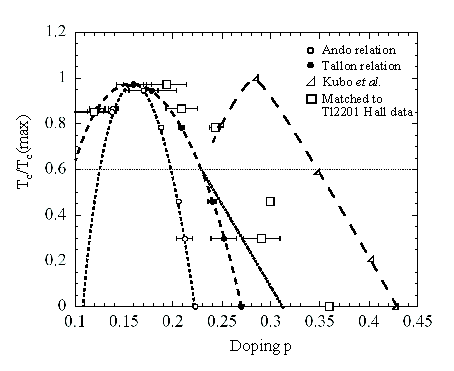
\includegraphics[scale=1.1]{Chapter-HallBSCO/Figures/Dopings/Dopings}
        \caption{Doping distributions for the three different methods. From left to right, B28KUD3A, B30KUD3 (Assume UD), B32KOP1, B32KOP4, B30KUD3 (Assume OD), B30KOD3, B16KOD1A, B07KOD2, B00KOD1A. Broken lines are a guide to the eye. Circled points are B30KUD3 for both the overdoped and underdoped scenarios.}
        \label{Fig:ResH:Dopings}
    \end{center}
\end{figure}

Figure~\ref{Fig:ResH:Rh300Comparison} present Hall data at \unit{300}{\kelvin} again taken in the Polo with comparable data from Konstantinovi\'c \etal~\cite{Konstantinovic2001}.
\begin{figure}[htbp]
    \begin{center}
        \includegraphics[scale=1.0]{Chapter-HallBSCO/Figures/Rh300Comparison/Rh300Comparison}
        \caption{Hall data at \unit{300}{\kelvin} compared with similar data taken from ref~\cite{Konstantinovic2001} using different doping assignments. From left: Tallon relation, Ando relation and scaling to \ac{TL2201} data. Red lines are guides to the eye, circled points are B30KUD3 in the overdoped and underdoped positions.}
        \label{Fig:Rh300Comparison}
    \end{center}
\end{figure}
It is clear that the Ando assignment of dopings is too confined with the data not at all following the respective curve whereas the Tallon relation follows much close the shape of the curve, although, perhaps this is not surprising given that the dopings in the Konstantinovo\'c paper were also assigned using the Tallon relation. However what is most interesting is that of the three methods, the scaling to the \ac{TL2201} \ac{dHvA} data gives the smoothest extrapolation. We continue assuming that the \ac{TL2201} doping assignments are the correct ones.

Also, referring to the circled points, we see that again the data is more consistent if we consider the B30KUD3 to be overdoped rather than underdoped. Looking back to the inset of figure~\ref{Fig:ResH:TSweeps} we see that there is large scatter in the data points due to uncertainty in the dimensions which were determined by optical microscope, however there is an approximate downward trend with doping which is similar to what is found in the literature~\cite{Ando2000, Ando1999, Konstantinovic2001, Ono2000}. Although B30KUD3 is more consistent to this trend in the underdoped position, the trend still lies with the error bars of the overdoped position. Looking ahead to the inset of figure~\ref{Fig:ResH:InvHallCombined} which shows $R_H$ values at \unit{300}{\kelvin} vs. doping, which depend only on the measurement of depth --- which was much more accurately determined by the \ac{FIB} --- we see that the underdoped position lies far outside the overall trend even when considering the error bars. 

